\pagebreak
\section{Appendix}
\begin{figure}[H]
    \centering
    \begin{subfigure}{2.1in}
        \centering
        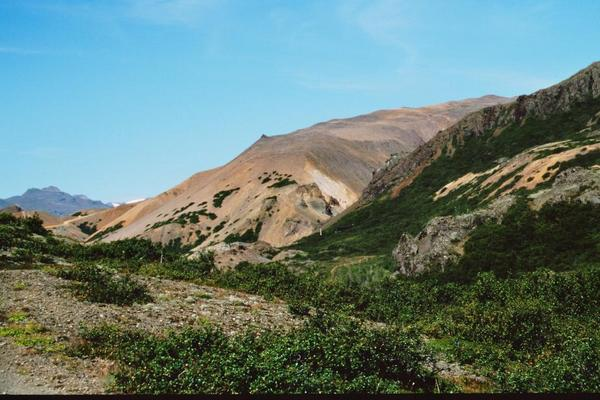
\includegraphics[width=2in]{./Images/mountain_color.jpg}
        \caption{(\textbf{a})}
    \end{subfigure}
    \begin{subfigure}{2.1in}
        \centering
        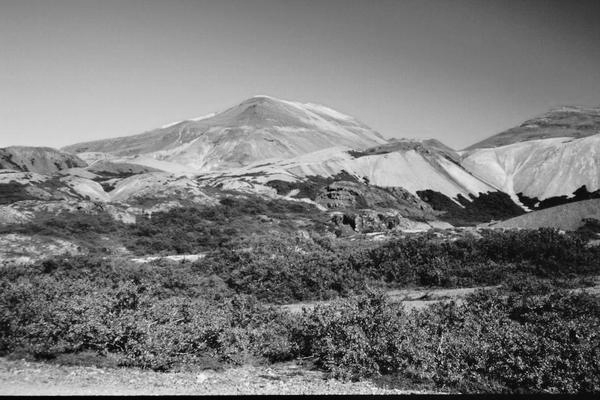
\includegraphics[width=2in]{./Images/mountain_gray.png}
        \caption{(\textbf{b})}
    \end{subfigure}
    \begin{subfigure}{2.1in}
        \centering
        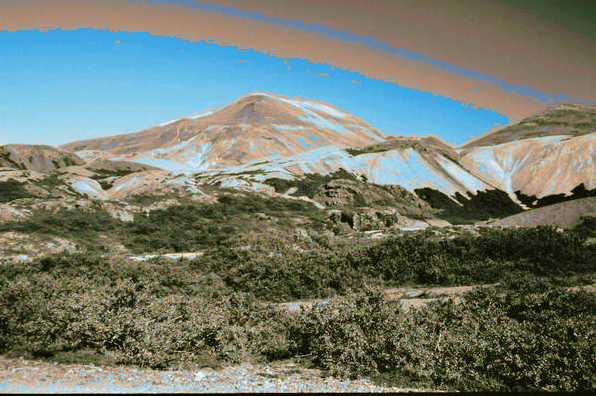
\includegraphics[width=2in]{./Images/mountain_gray_colored_40.png}
        \caption{(\textbf{c})}
    \end{subfigure}
    \caption{The baseline colorization procedure. (\textbf{a}) A colored training image. (\textbf{b}) A gray-scale test image. (\textbf{c})  A colorized version of the test image.}
    \label{fig:baseline_result}
\end{figure}

\begin{figure}[H]
    \centering
    \begin{subfigure}{2.1in}
        \centering
        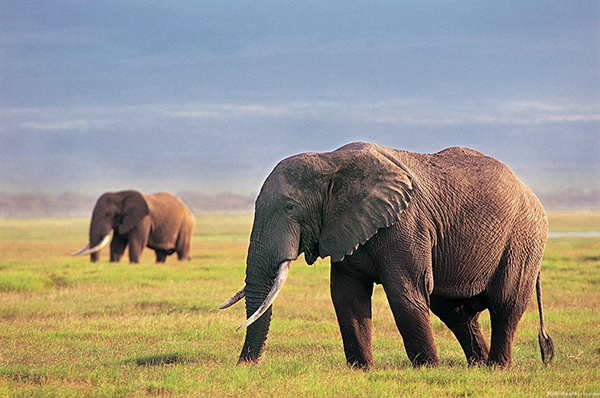
\includegraphics[width=2in]{./Images/elephant2.jpg}
        \caption{(\textbf{a})}
    \end{subfigure}
    \begin{subfigure}{2.1in}
        \centering
        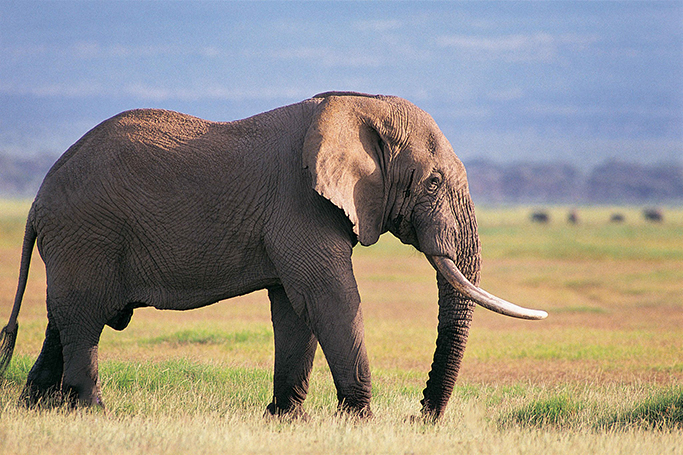
\includegraphics[width=2in]{./Images/elephant1.jpg}
        \caption{(\textbf{b})}
    \end{subfigure}
    \begin{subfigure}{2.1in}
        \centering
        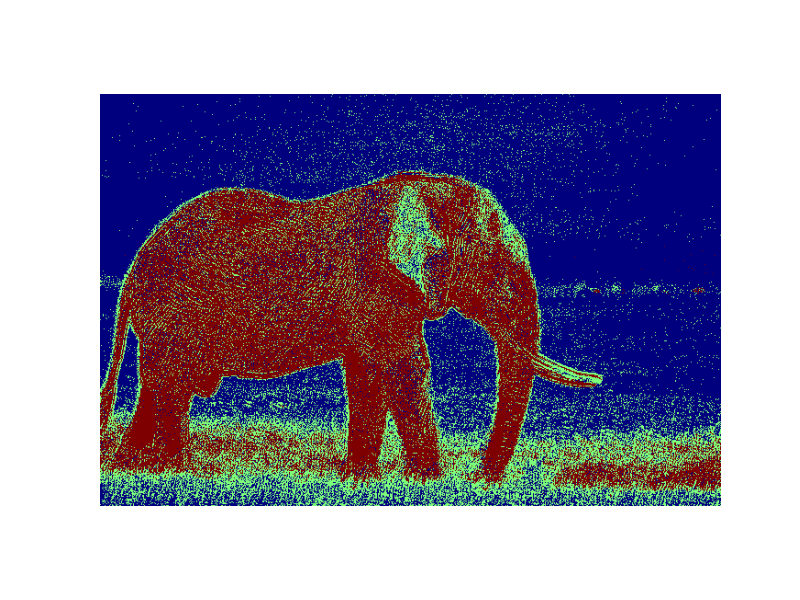
\includegraphics[width=2in]{./Images/2.png}
        \caption{(\textbf{c})}
    \end{subfigure}
    \newline
    \begin{subfigure}{2.1in}
        \centering
        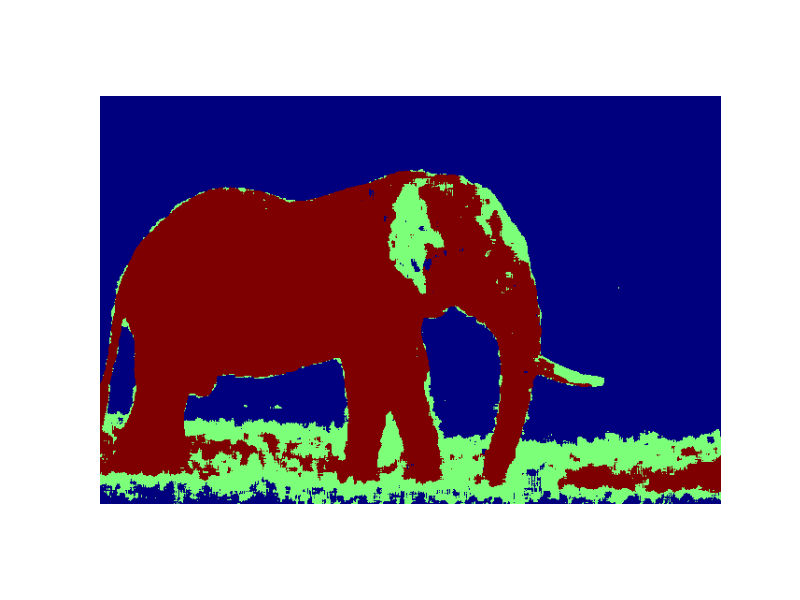
\includegraphics[width=2in]{./Images/3.png}
        \caption{(\textbf{d})}
    \end{subfigure}
    \begin{subfigure}{2.1in}
        \centering
        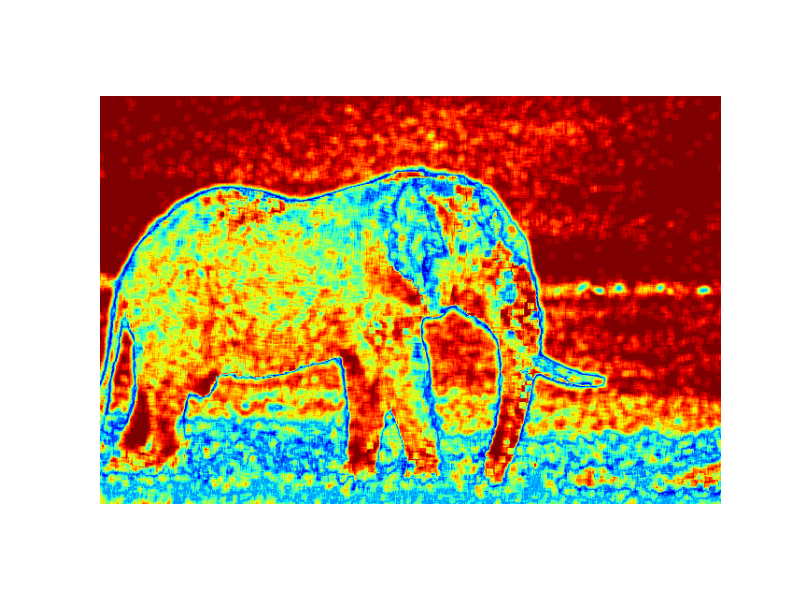
\includegraphics[width=2in]{./Images/4.png}
        \caption{(\textbf{e})}
    \end{subfigure}
    \begin{subfigure}{2.1in}
        \centering
        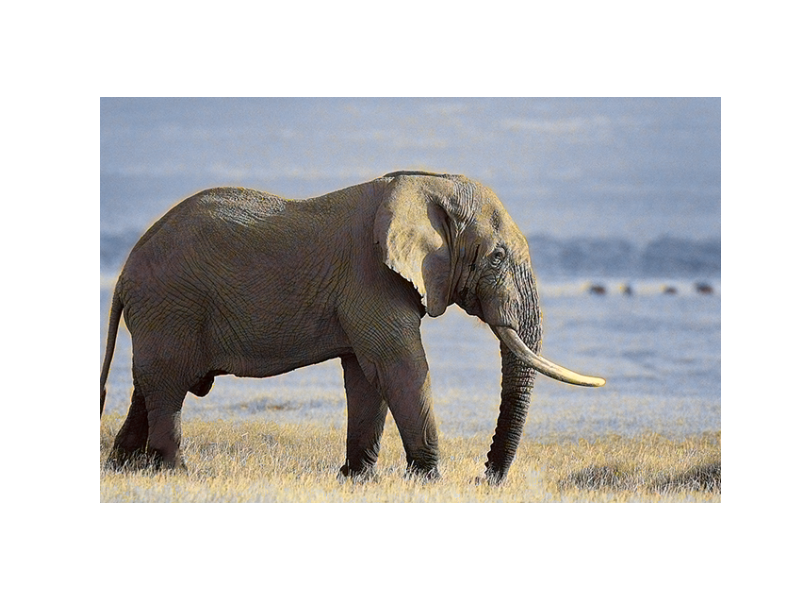
\includegraphics[width=2in]{./Images/5.png}
        \caption{(\textbf{f})}
    \end{subfigure}
    \caption{The more complicated colorization procedure. (\textbf{a}) A colored training image. (\textbf{b}) The test image with the orginal color. (\textbf{c})  The results of running kNN on the test image. (\textbf{d})  The results of image-space voting on the kNN results. (\textbf{e})  The confidence of each pixel's prediction. (\textbf{f})  The colorized version of the test image.}
    \label{fig:elephants}
\end{figure}

\begin{figure}[H]
    \centering
    \begin{subfigure}{3.1in}
        \centering
        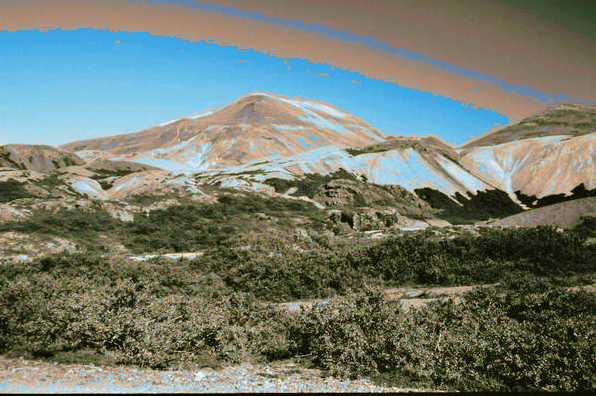
\includegraphics[width=3in]{./Images/mountain_gray_colored_40.png}
        \caption{(\textbf{a})}
    \end{subfigure}
    \begin{subfigure}{3.1in}
        \centering
        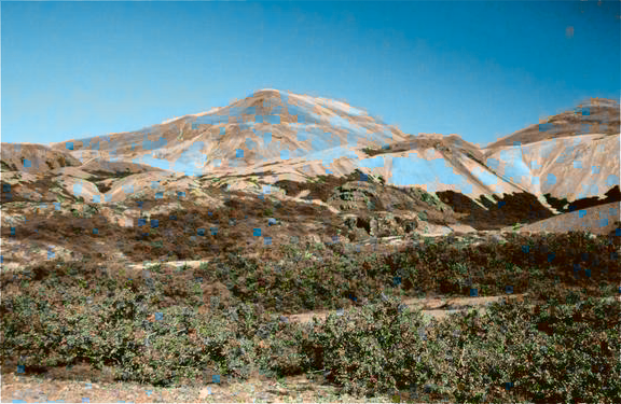
\includegraphics[width=3in]{./Images/landscape_5.png}
        \caption{(\textbf{b})}
    \end{subfigure}
    \caption{A comparison of our baseline and more complicated colorization results. (\textbf{a}) The baseline colorization. (\textbf{b}) Our more complex colorization.}
    \label{fig:algo_compare}
\end{figure}